% !TeX spellcheck = en_US
\addsection{Player Turns}{\spells/dimension_door.png}

\begin{multicols}{2}

At the start of your Turn, refresh your hand of Cards following these steps:
\begin{itemize}
  \item Discard any number of Cards from your hand.
If your current hand exceeds your Hand Limit \includesvg[height=10px]{\svgs/hand.svg}, you must discard down to match the Limit.
  \item You may then draw Cards up to your Hand Limit.
  \item Resolve any "at the beginning of your turn" abilities after drawing.
\end{itemize}
Your current Hand Limit\index{Hand Limit} depends on your Main Hero's \hyperlink{Level}{Level}.
The beginning of your Turn is the only time your Hand Limit is checked.\par
There are three types of Actions players may take: \textbf{Movement}, \textbf{Town}, and \textbf{Morale}.
Once all players have spent all their Movement Points and do not wish to use any further Town or Morale Actions, the current Round is over.

\subsection*{Movement Actions}
\hypertarget{Movement}{Movement Actions}\index{Movement Actions} are performed by spending Movement Points.
A player can use Movement Actions \textbf{only during their own Turn}.\par
For every 1 MP spent, you can perform one of the following Actions:
\begin{itemize}
  \item Move a Hero 1 Field in any direction.
  \item \hyperlink{Categories}{Revisit} a Field where your Hero is in.
  \item \hyperlink{Timelimit}{Continue Combat} against Neutral Units for 1 additional Combat Round.
  \item \hyperlink{Placing}{Discover a face down Map Tile} if your Hero is on a Field next to that Tile.
  \item Place a new Map Tile from your pool of Far (II–III) Map Tiles.
\end{itemize}

\begin{center}
  \includesvg[width=0.6\linewidth]{\images/movement_tokens.svg}\\
  \medskip
  \footnotesize\textit{An active and an inactive Movement Token.}
\end{center}

\bigskip

Mark the amount of MP you have used by flipping your Movement Tokens over to their brown, inactive side.
If a player has both a Main and a \hyperlink{Secondary}{Secondary Hero}, track their MPs separately.
Heroes can spend MP in any order.\par
Allied Heroes can move through each other but cannot stop their movement in the same Field.
When you move through a Field with an allied Hero, do not \hyperlink{Categories}{Visit} the Field that the allied Hero is standing on.\par

\note{10}{
  Whenever you are instructed to gain (additional) MP, sometimes represented by the symbol \includesvg[height=10px]{\svgs/movement-note.svg}, that MP persists for \textbf{only the Turn it was gained on}.
  In the unlikely situation that two allied Heroes are forced onto the same Field, you must use your next MP to move one of them away from that Field.
}

\vfill
\begin{center}
  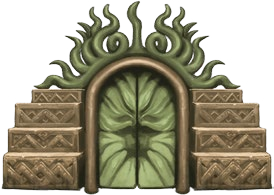
\includegraphics[width=0.8\linewidth]{\art/town_portal.png}
\end{center}

\clearpage

\subsection*{Town Actions\index{Town Actions}}
You can perform each of the Town Actions listed below \textbf{once per Round}.
These Actions can be performed at any point during any player's Turn, except during Combat or when your Town Action would interrupt another Action.
For example, you cannot draw Spell cards simultaneously with the Spell Book Token.\par
When a player announces that they are about to start Combat, you may react to it with any number of Town Actions before performing any of the steps of \hyperlink{Combatsetup}{setting up Combat.}\par
After performing a Town Action, flip the respective Token on its inactive side on your Town Board.
You cannot use that Action again until the start of the next Round, when the Tokens are refreshed.
\begin{itemize}
  \item [{
\includegraphics[height=1.5\baselineskip, valign=c]{\images/build.png}}] Build Token, used to expand your \hyperlink{Town}{Town}.
  \item [{
\includegraphics[height=1.5\baselineskip, valign=c]{\images/population.png}}] Population Token, used to Recruit and Reinforce \hyperlink{Units}{Units} or to Recruit \hyperlink{Secondary}{a Secondary Hero}.
  \item [{
\includegraphics[height=1.5\baselineskip, valign=c]{\images/spells.png}}]Spell Book Token, used to purchase \hyperlink{spells}{Spells}. Requires the Mage Guild Town building to use.
\end{itemize}

\subsection*{Morale Actions}\index{Morale Actions}
Players can gain or lose Morale through various game effects.
When you gain Morale, take a Positive Morale Token\index{Positive Morale} \includesvg[height=10px]{\svgs/morale_positive.svg}.
You may only have one such Token.
If you are about to gain a second Token, you may immediately spend the first one before gaining the second.
A Positive Morale Token may be spent to perform any of the following Actions at any time:
\begin{itemize}
  \item Draw a Card from your Deck.
  \item Discard any number of Cards, then draw that many Cards.
  \item Reroll any Die you have thrown.
\end{itemize}
If you lose Morale, discard a Positive Morale Token \includesvg[height=10px]{\svgs/morale_positive.svg} if you have one, otherwise gain a Negative Morale\index{Negative Morale} Token \includesvg[height=10px]{\svgs/morale_negative.svg}.
Inversely, gaining Positive Morale while you have a Negative Morale Token discards the Token.
If you would gain a second Negative Morale Token, you must instead \textbf{discard your hand of Cards} the next time you end your Turn.\par

\note{5}{The Necropolis \includesvg[height=10px]{\svgs/necro-note.svg} Faction ignores any Morale effects.
  They cannot ever gain or lose Morale for any reason.
}

\begin{center}
  \makebox[\linewidth]{
\includegraphics[width=1.1\linewidth]{\art/shield.png}}
\end{center}

\subsection*{Example Turn}

\textit{Alice, who is playing the Hero Catherine the Knight, begins her Turn.
She has 3 cards in her hand from the previous round, and decides to discard 2 of them before drawing cards from her Deck up to her Hand Limit \includesvg[height=10px]{\svgs/hand.svg}.
The current limit is 5, since her Main Hero is Level 3, so she draws 4 cards after discarding (see \hyperlink{Level}{Level Effects}).}\par
\textit{She then spends her Build Token to construct the \includesvg[height=10px]{\svgs/golden.svg} Dwelling, and then her Population Token to \hyperlink{Units}{Recruit} the \includesvg[height=10px]{\svgs/golden.svg} Unit Champions.
She can do this, as she had previously built the prerequisite lower Level Dwellings (\includesvg[height=10px]{\svgs/bronze.svg} and \includesvg[height=10px]{\svgs/silver.svg}) and has enough \hyperlink{Resources}{Resources} to both Build the Dwelling and to Recruit the Champions.}\par
\textit{Now prepared for a upcoming battle, she spends a Movement Point to move her Main Hero to an adjacent Field currently occupied by Sandro the Necromancer, an enemy Main Hero controlled by Bob.
As Alice announces her intent to start Combat, both players still have an opportunity to perform Town Actions.}\par

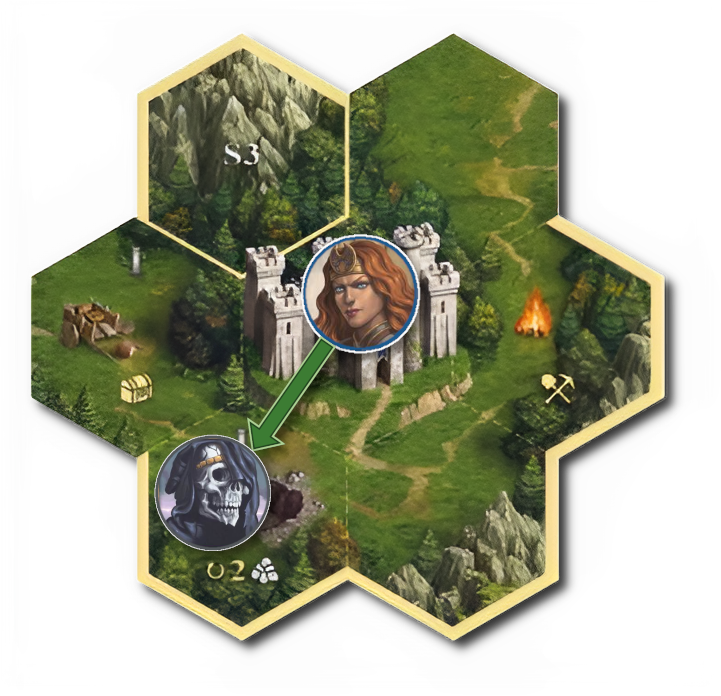
\includegraphics[width=\linewidth]{\examples/catherine_attacks_sandro.png}

\end{multicols}

\vfill

\begin{scaledfigure}[blanker]
 \centering
 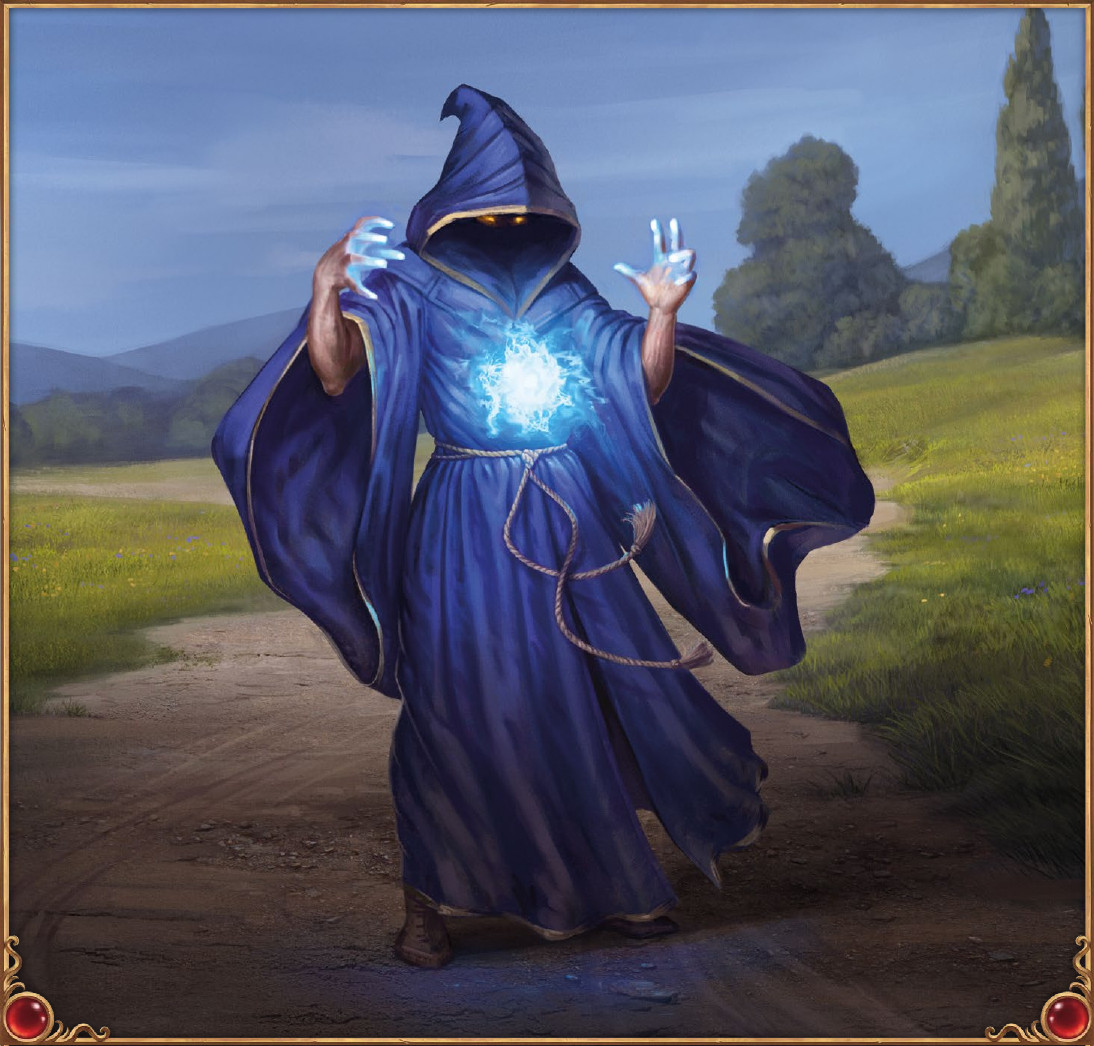
\includegraphics[width=\linewidth, height=\myspace, keepaspectratio]{\art/zealot.jpg}
\end{scaledfigure}
